\documentclass[border=6pt]{standalone}
\usepackage{tikz}
\usetikzlibrary{arrows.meta,positioning}
\begin{document}
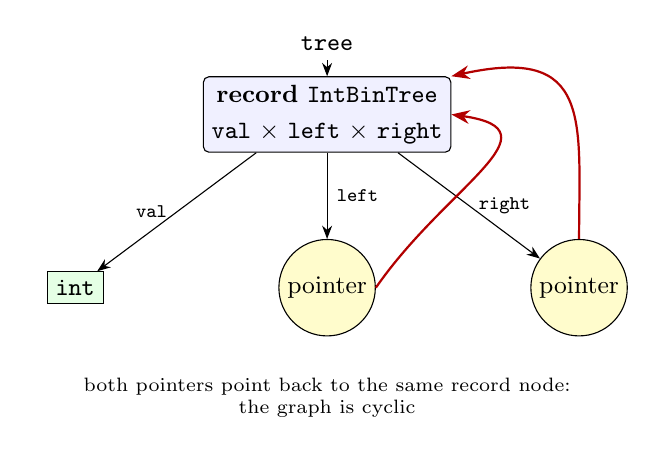
\begin{tikzpicture}[>=Stealth,font=\small,
  rec/.style={draw,rounded corners=2pt,fill=blue!6,inner sep=3pt,minimum width=2.6cm},
  pt/.style={draw,circle,inner sep=2pt,fill=yellow!20},
  bt/.style={draw,rectangle,inner sep=3pt,fill=green!10}]
\node[rec,align=center] (r) at (0,0) {\textbf{record}\ \texttt{IntBinTree}\\[2pt] \texttt{val} $\times$ \texttt{left} $\times$ \texttt{right}};
\node[bt] (i) at (-3.2,-2.2) {\texttt{int}};
\node[pt] (p1) at (0,-2.2) {pointer};
\node[pt] (p2) at (3.2,-2.2) {pointer};
\node[font=\scriptsize,above left=0.02cm and 0cm of i] {};
\draw[->] ([xshift=-0.9cm]r.south) -- node[left,font=\scriptsize]{\texttt{val}} (i);
\draw[->] (r.south) -- node[right,font=\scriptsize]{\texttt{left}} (p1);
\draw[->] ([xshift=0.9cm]r.south) -- node[right,font=\scriptsize]{\texttt{right}} (p2);
\draw[->,thick,red!70!black] (p1.east) .. controls +(0.9,1.3) and +(1.4,-0.2) .. (r.east);
\draw[->,thick,red!70!black] (p2.north) .. controls +(0,1.5) and +(1.8,0.4) .. (r.north east);
\node[font=\scriptsize,align=center,below=0.4cm of p1] {both pointers point back to the same record node:\\the graph is cyclic};
\node[above=0.2cm of r,font=\small] {\texttt{tree}};
\draw[->] ([yshift=0.2cm]r.north) -- (r.north);
\end{tikzpicture}
\end{document}
